\documentclass[11pt]{article}
\usepackage[letterpaper]{geometry}
\usepackage{times}
\usepackage{verbatim}
\usepackage{graphicx}
\usepackage{float}
\usepackage{fullwidth}
\usepackage{amsmath}
\usepackage{amssymb}
\usepackage{fourier}
\usepackage{hyperref}
\graphicspath{{Images/}}
\title{ENGR-241 Passive Filters Lab}
\author{Jeremy Munson, Lauren Speirs \& Andrew Henrikson}
\geometry{top=.8in, bottom=.8in, left=.8in, right=.8in}

\setlength{\parindent}{0em}
\setlength{\parskip}{.5em}
\begin{document}
	\maketitle
	\subsection*{Overview}
	For this lab we designed and  constructed an active Butterworth Low Pass Filter with a cutoff frequency of 1KHz and a passband gain of 6 dB. The circuit was designed to have a minimum of 70dB of attenuation at 10KHz. We disgned and tested the circuit using Orcad prior to building the circuit. We then built and observed the output on the oscilloscope to ensure we met the design requirements.
	\subsection*{Circuit Diagrams}
		\begin{figure}[H]
		\centering
		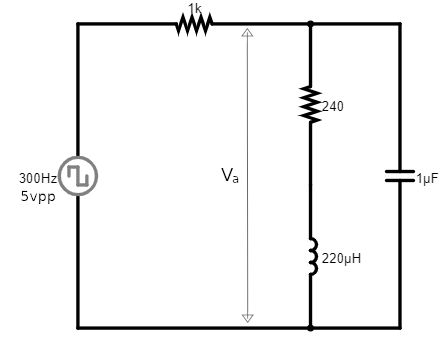
\includegraphics[width=5.5in]{images/diagram.PNG}
	\end{figure}
	\subsection*{Calculations}
	The calculations for this lab required us to determine the number of stages needed to meet the attenuation specifications of 70dB at 10KHz. We then calculated the values for the capacitors using scaling and choosing a resistor value of 1k $\Omega$.
	\subsubsection*{1. Approximate the number of stages needed to attain 70dB of attenuation.}
	Given:\\
	$f_{s}=10KHz$\\
	$f_{p}=1KHz$\\\\
	$n=\frac{-0.05A_{s}}{log(f_{s}/f_{p})}$\\
	$n=\frac{-0.05\cdot -70}{log(10KHz/1KHz)}=3.5$\\\\
	=>four stages should provide the required attenuation
	\subsubsection*{2. Using the roots from the Butterworth $n^{th}$ order polynomial table, calculate the roots of the polynomials for a fourth order filter.}
	Given:
	$(s^{2}+0.765s+1)(s^{2}+1.848s+1)$\\
	$C_{1}=2.61F$\\
	$C_{2}=0.38F$\\
	$C_{3}=1.08F$\\
	$C_{4}=0.924F$\\
	\subsubsection*{3. Using the values found above, scale the capacitors for the selected resistor value.}
	
	$R'=k_{m}R=1k\Omega$\\
	$k_{f}= \frac{\omega'_{c}}{\omega_{c}}=2000\pi$\\\\
	$C'=\frac{C}{k_{m}k_{f}}$\\
	$C'_{1}=\frac{C_{1}}{k_{m}k_{f}}=\frac{2.614F}{2000\pi\cdot1000}=416.0nF$\\
	$C'_{2}=\frac{C_{2}}{k_{m}k_{f}}=\frac{0.3825F}{2000\pi\cdot1000}=60.9nF$\\	
	$C'_{3}=\frac{C_{3}}{k_{m}k_{f}}=\frac{1.08F}{2000\pi\cdot1000}=171.9nF$\\ 
	$C'_{4}=\frac{C_{4}}{k_{m}k_{f}}=\frac{0.924F}{2000\pi\cdot1000}=147.1nF$\\ 
	\subsection*{Data Table}
		\begin{table}[H]
		\def\arraystretch{1.2}%
		\centering
		\begin{tabular}{|l|l|l|l|}
			\hline
			Frequency(Hz)		& $V_{out}$(ideal)		&  $V_{out}$(observed) 			&\% Diff	\\ \hline
			100  				& $10V$						& $10.05V$        			&0.5\%		\\ \hline	
			250					& $10.1V $					& $10.0V $    				&-0.99\%	\\ \hline
			500					& $10.3V$					& $9.6V$					&-6.80\%	\\ \hline
			600					& $10.3V$					& $9.25V$					&-10.19\%	\\ \hline
			700					& $10.2V$					& $8.75V$					&-14.22\%	\\ \hline
			800					& $9.6V$					& $8V$						&-16.67\%	\\ \hline
			900					& $8.5V$					& $7V$						&-17.65\%	\\ \hline
			1k					& $7V$						& $5.7V$					&-11.63\%	\\ \hline
			1.1k				& $5.4V$					& $4.6V$					&-8.0\%		\\ \hline
			1.2k				& $4V$						& $3.65V$					&-8.75\%	\\ \hline
			1.3k				& $3V$						& $2.8V$					&-6.67\%	\\ \hline
			1.5k				& $1.8V$					& $1.9V$					&5.56\%		\\ \hline
			2k					& $530mV$					& $700mV$					&32.07\%	\\ \hline
			3k					& $111mV$					& $200mV$					&80.2\%		\\ \hline
			4k					& $33mV$					& $75mV$					&127\%		\\ \hline
			5.5k				& $10mV$					& $32.5mV$					&225\%		\\ \hline
			
			
			
			
			
	\end{tabular}
	\end{table}
\end{document}